\documentclass[
	11pt,
	a4paper,
	bibtotocnumbered
	]{scrreprt}		                                   


% ---------- Encoding and Language ----------

\usepackage[utf8]{inputenc}

\usepackage[ngerman]{babel}
\usepackage[babel,german=quotes]{csquotes}

% ---------- Maskierung von URLs und Dateipfaden ----------
\usepackage[hyphens]{url}

% ---------- Abbildungen ----------
\usepackage{graphicx}
\usepackage[dvipsnames]{xcolor}
\usepackage{a4}
\usepackage{caption}

% ---------- Schriften ----------
\usepackage[onehalfspacing]{setspace}

% ---------- Math ----------
\usepackage{mathtools}
\usepackage{amsmath}
\usepackage{amssymb}

% ---------- Listings ----------
\usepackage{listings}
\definecolor{javared}{rgb}{0.6,0,0} % for strings
\definecolor{javagreen}{rgb}{0.25,0.5,0.35} % comments
\definecolor{javapurple}{rgb}{0.5,0,0.35} % keywords
\definecolor{javadocblue}{rgb}{0.25,0.35,0.75} % javadoc

% global listing settings
\lstdefinestyle{myNumbers} {
	numbers=left,
	numberstyle=\tiny\color{black},
	stepnumber=1,
	numbersep=5pt
}
\lstdefinestyle{myFrame} {
	backgroundcolor=\color{white},
	frame=lines
}
\lstdefinestyle{myStyle} {
	tabsize=2,
	basicstyle=\ttfamily\small,
	breaklines=true,
	prebreak=\raisebox{0ex}[0ex][0ex]{\ensuremath{\hookleftarrow}},
	breakautoindent=true,
	showtabs=false,
    showspaces=false,
    showstringspaces=false,
}

% Java Style
\lstdefinestyle{myJavaStyle} {
	language=java,
 	keywordstyle=\color{javapurple}\bfseries,
   	stringstyle=\color{javared},   
   	commentstyle=\color{javagreen},
    morecomment=[s][\color{javadocblue}]{/**}{*/},
    style = myStyle,
    style = myFrame,
    style = myNumbers
}

% C Style
\lstdefinestyle{myCppStyle} {
	language=C++,
 	keywordstyle=\color{blue}\bfseries,
   	stringstyle=\color{gray},   
   	commentstyle=\color{green},
   	style = myStyle,
    style = myFrame,
    style = myNumbers
} 

% ---------- Misc ----------
\usepackage[printonlyused]{acronym}
\usepackage[linktoc=all, hidelinks]{hyperref}
\usepackage{booktabs}

% ---------- Bibliography ----------
\usepackage[backend=biber, hyperref=true]{biblatex}
\addbibresource{bibliography.bib}

\captionsetup[table]{belowskip=8pt}


\begin{document}



% ============================ FRONT MATTER
\pagenumbering{Roman}
\begin{singlespace}
\begin{titlepage}

\vspace*{-3.5cm}

\begin{flushleft}
\hspace*{-1cm} 
\includegraphics[width=15.7cm]{htwg-logo}
\end{flushleft}

\vspace{2.5cm}

\begin{center}
	\huge{
		\textbf{Visualisierungs-Framework für graphische Algorithmen, insbesondere Subdivision} \\[5cm]
	}
	\Large{
		\textbf{Tobias Keh, Simon Kessler, Felix Born}} \\[6.5cm]
	\large{
		\textbf{Konstanz, 01.07.2015} \\[2.3cm]
	}
	
	\Huge{
		\textbf{{\sf PROJEKTARBEIT}}
	}
\end{center}

\end{titlepage}
\setcounter{page}{1}
\end{singlespace}

\tableofcontents

\cleardoublepage
% ============================ ENDE FRONT MATTER


% ============================ HAUPTTEIL
\pagenumbering{arabic}


% ============================ CHAPTERS

Anforderungen an den Bericht
- technischer Bericht
- einfache Sätze
- Verwendung von Nebensätzen nur spärlich
- Definition eines Begriffs bei erster Verwendung
- konsequente Verwendung der selben Begriffe, keine Änderung im Text (keine Synonyme)
- Verwendung von Gegenwart
- Aktiv oder Passiv (konsistent)
- Anreicherung des Texts mit wichtigen Codestellen (Highlights, wichtige Entscheidungsstellen), Bildern und Tabellen
- jeweils mit ausführlicher Beschreibung an entsprechender Stelle
- Zitate mit Nummern oder vollen Namen und Jahreszahl
- ausführliche Dokumentation / Benutzerhandbuch 
- Installationsanleitung (spezielle Abhängigkeiten, etc.)
- Deployment / Installation
- Beispielplugin, wie werden sie registriert etc.
- Memory Management

\chapter{Einführung}

Unterteilung beschreibt das Verfahren, aus einem Ausgangspolygonnetz eine glatte Fläche zu erzeugen.
Dadurch lassen sich durch ein Kontrollnetz Flächen beliebiger Form beschreiben.

Das Ziel dieses Projekts ist es ein Programm zu entwickeln, welches ausgewählte Unterteilungsalgorithmen implementiert.
Es soll ein beliebiges Kontrollnetz geladen und editiert werden können.
Das Programm soll die Fläche rendern und die Unterteilungsalgorithmen auf das Kontrollnetz anwenden können.

Dieses Dokument definiert die Anforderungen an das Programm und evaluiert verschiedene Bibliotheken und Datenstrukturen, die später für das Projekt verwendet werden sollen.
\chapter{Grundlagen}


\section{Subdivison Übersicht}

Subdivison Algorithmen erzeugen aus einem Ausgangspolygonnetz eine glatte Fläche.
Die glatte Zielfläche ist dabei der Grenzwert eines unendlichen, rekursiven Verfeinerungsschemas.
Abbildung~\ref{fig:sd} visualisiert die Anwendung eines Subdivison Algorithmus auf eine Kurve und auf eine Fläche.
Nach mehrfacher Anwendung der Unterteilung konvergiert die Kurve oder Fläche gegen die glatte Zielkurve bzw. Zielflähe.
\begin{figure}[h]
  \caption{Subdivison Algorithmus - Kurve und Fläche}
  \centering
  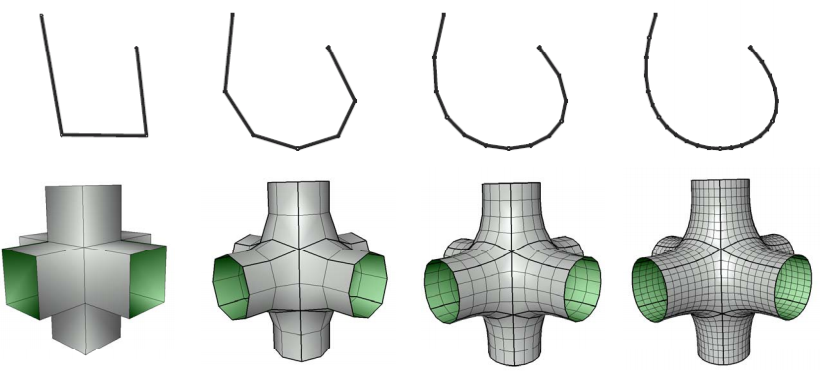
\includegraphics[width=0.8\textwidth]{content/media/sd.png}
  \\Quelle: \cite{Standford.24.07.2015}
  \label{fig:sd}
\end{figure}

Subdivision Algorithmen kann man anhand ihrer Eigenschaften Kategorisieren.
Ein Unterscheidungskriterium betriefft die Art und Weiße, wie unterteilt wird.
Man unterscheidet dabei zwischen \emph{Primal} und \emph{Dual}.
\begin{description}
 \item[Primal] Bei dieser Strategie wird die Oberfläche unterteilt ("face slit").
 Abbildung~\ref{fig:sd_primal} stellt diese Methode für ein Dreicksnetz und ein Vierecksnetz dar.
 \item[Dual] Auf der anderen Seite ist es möglich Eckpunkte in mehrere Eckpunkte aufzusplitten ("vertex split").
 Diese Methode ist in Abbildung~\ref{fig:sd_dual} abgebildet.
\end{description}
\begin{figure}[h]
  \caption{Primal (Face Split)}
  \centering
  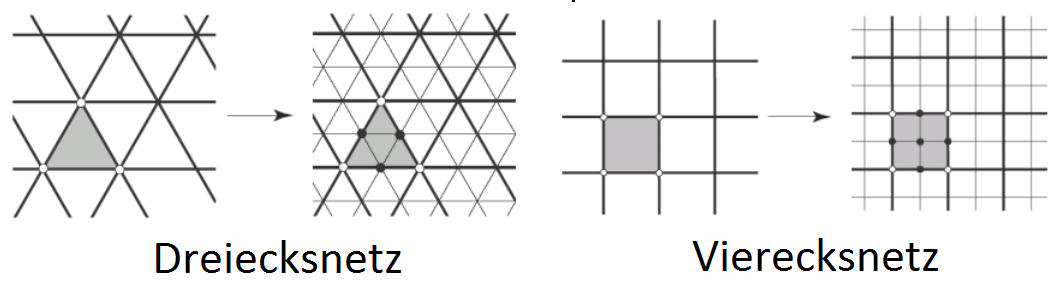
\includegraphics[width=0.7\textwidth]{content/media/sd_primal}
  \\Quelle: \cite{Standford.24.07.2015}
  \label{fig:sd_primal}
\end{figure}
\begin{figure}[h]
  \caption{Dual (Vertex Split)}
  \centering
  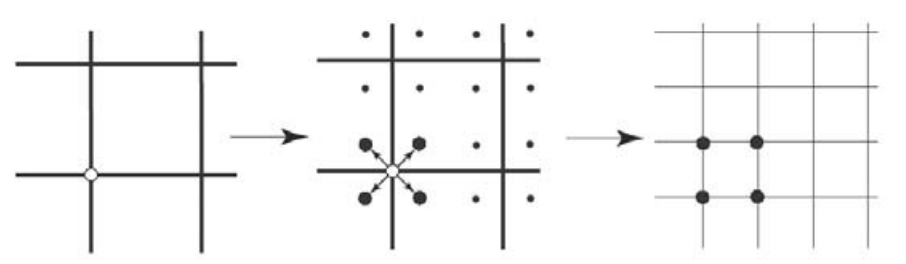
\includegraphics[width=0.7\textwidth]{content/media/sd_dual}
  \\Quelle: \cite{Standford.24.07.2015}
  \label{fig:sd_dual}
\end{figure}

Ein weiteres wesentliches Merkmal ist, ob Kontrollpunkte interpoliert werden oder nicht. 
\begin{description}
 \item[Approximation] Kontrollpunkte werden nicht interpoliert.
 \item[Interpolation] Kontrollpunkte werden interpoliert.
\end{description}

Tabelle~\ref{tab:sd_comp} listet die bekanntesten Subdivison Algorithmen auf und ordnet diese den Kategorien zu.
Zu jedem Algorithmus ist zusätzlich die "Glattheit" der Oberfläche angegeben (C-Stetigkeit).
Dies kann auch als Maß über die Qualität des Subdivision Algorithmus fungieren.
\begin{table}[h]
\caption{Subdivison Zoo}
\center
\begin{tabular}{|l|c|c|c}
\toprule
\multicolumn{3}{c|}{\textbf{Primal}} & \textbf{Dual}\\
\midrule
& \textbf{Dreiecksnetz} & \textbf{Vierecksnetz} & \\
\midrule
\textbf{Approximation} & Loop \((C^2)\) & Catmull-Clark \((C^2)\) & Doo-Sabin \((C^1)\) \\
\textbf{Interpolation} & Butterfly \((C^1)\) & Kobbelt \((C^1)\) & Biquartic \((C^2)\) \\
\bottomrule
\end{tabular}
\label{tab:sd_comp}
\end{table}

Abbildung~\ref{fig:sd_comp} Vergleicht die 4 unterschiedlichen Subdivison Algorithmen.
Man erkennt deutlich den interpolierenden Subdivison Algorithmus (Butterfly),
da dieser durch die harten Interpolationsbedingungen im Vergleich zu den approximierenden Algorithmen viel welligere ist.
\begin{figure}[h]
  \caption{Vergleich der Subdivison Algorithmen}
  \centering
  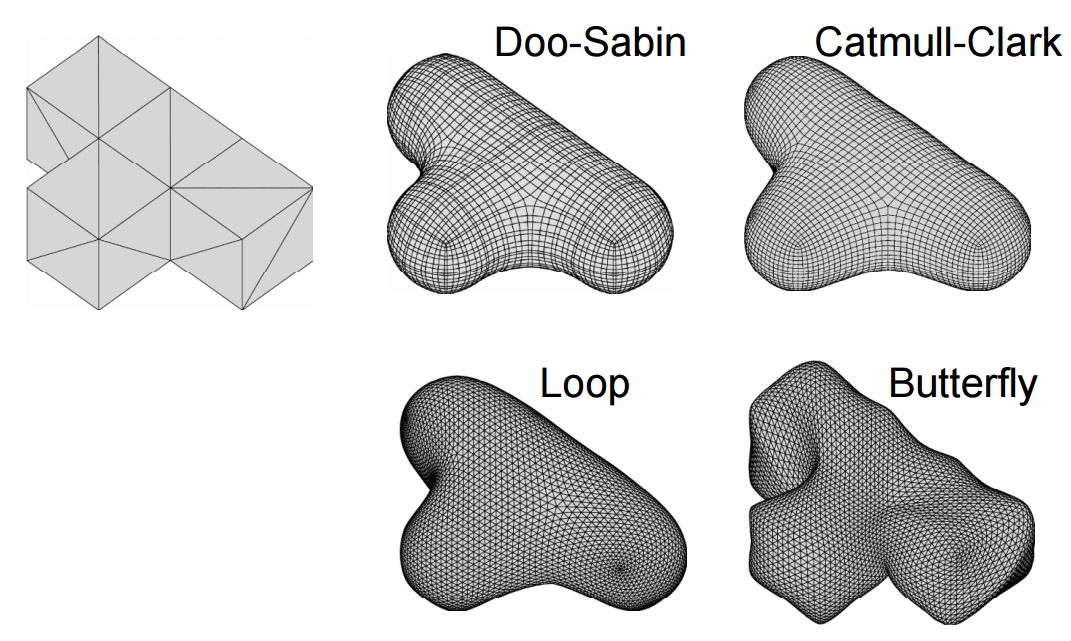
\includegraphics[width=0.9\textwidth]{content/media/sd_overview.png}
  \\Quelle: \cite{Standford.24.07.2015}
  \label{fig:sd_comp}
\end{figure}

\section{Auswahl der Subdivison Algorithmen}

Für das Projekt sollen folgende Algorithmen implementiert werden:
\begin{itemize}
	\item Catmull-Clark
	\item Loop
	\item Doo-Sabin
	\item Butterfly
\end{itemize}



\chapter{Tools und Bibliotheken}

In diesem Kapitel werden Bibliotheken und Programme untersucht, die für das Projekt verwendet werden können. 
 
\section{Unterteilungsalgorithmen und Datenstrukturen}

Im Bereich Unterteilungsalgorithmen gibt es viele bereits implementierte Datenstrukturen und Algorithmen.
Gesucht wird eine einfache Datenstruktur, um Polygonnetze verarbeiten zu können.
Diese sollte so wenig Overhead wie möglich mitbringen.
Im Allgemeinen besteht solch eine Datenstruktur aus Ecken (Vertices), Kanten (Edges) und Flächen (Faces).
Zusätzlich muss noch die Beziehung zwischen den Objekten abgespeichert werden.

\subsection{OpenMesh}

OpenMesh wird von der RWTH Aachen entwickelt und stellt eine mächtige Datenstruktur für Polygonnetze bereit.
Es steht unter der LGPL v3 Lizenz (\enquote{with exception}) und kann somit problemlos verwendet werden.

OpenMesh implementiert eine Datenstruktur für Polygonnetze.
Darüber hinaus sind bereits einige Unterteilungsalgorithmen implementiert, die auf der OpenMesh Datenstruktur arbeiten können.
Zum Funktionsumfang gehören folgende Algorithmen:

\begin{enumerate}
\item Uniform subdivision
\begin{itemize}
	\item Loop
	\item Sqrt3
	\item Modified Butterfly
	\item Interpolating Sqrt3
	\item Composite
	\item Catmull Clark
\end{itemize}
\item Adaptive subdivision
\begin{itemize}
	\item Adaptive Composite
\end{itemize}
\item Simple subdivision
\begin{itemize}
	\item Longest Edge
\end{itemize}
\end{enumerate}

OpenMesh implementiert eine \emph{Halfedge} Datenstruktur.
Diese \emph{kantenbasierte} Datenstrukturen speichern die Information über die Verbindungen zwischen Eckpunkten in den Kanten, während
\emph{flächenbasierte} Datenstrukturen die Verbindungsinformation zwischen den Eckpunkten und Nachbarn in den Flächen speichern.

Jede Kante referenziert also folgende Objekte:

\begin{itemize}
	\item zwei Eckpunkte
	\item eine Fläche
	\item die nächsten zwei Kanten der Fläche
\end{itemize}

Halfedge bedeutet nun, dass eine Kante in zwei Halbkanten (Halfedge) aufgeteilt wird. 
Jede Halbkante hat nur eine Richtung.
Zwei Ecken A und B sind also über zwei Halbkanten (erste Halkante von A nach B und zweite Halbkante von B nach A) miteinander verbunden.
Dies bringt den Vorteil, dass man über die Kanten einer Fläche sehr einfach iterieren kann. Man muss dazu lediglich den Halbkanten folgen.


\subsubsection{OpenFlipper}

Aufbauend auf OpenMesh wurde von der RWTH Aachen zusätzlich das flexible Plugin-basierte Framework OpenFlipper enwickelt.
Damit können geometrische Objekte modelliert und verarbeitet werden. Intern wird auf die Datenstrukur OpenMesh zurückgegriffen.
Für die grafische Oberfläche wird QT verwendet.
Mit OpenFlipper kann man über die Oberfläche Netze erstellen und die in OpenMesh implementierten Subdivision Algorithmen anwenden.
\autoref{fig:openflipper} zeigt die Benutzeroberfläche von OpenFlipper.

\begin{figure}
  \centering
  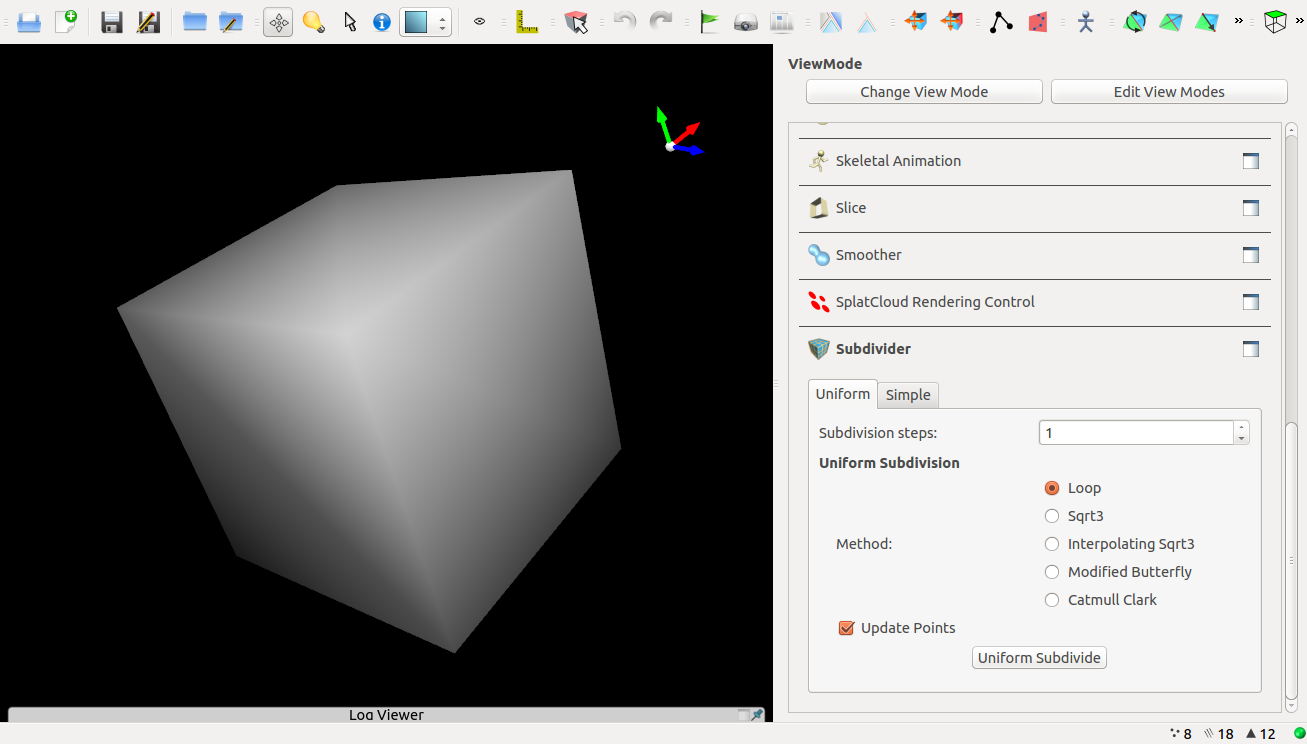
\includegraphics[width=0.8\textwidth]{content/media/openflipper_cube}
  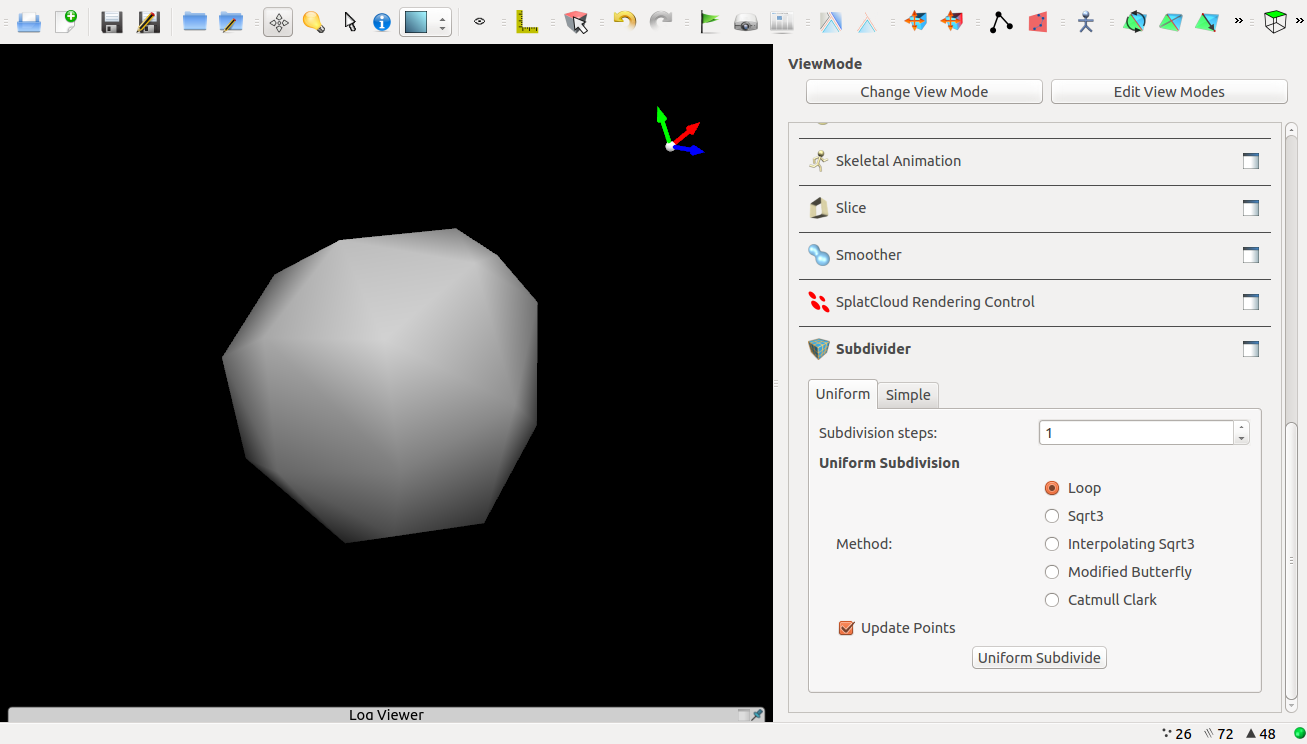
\includegraphics[width=0.8\textwidth]{content/media/openflipper_loop}
  \caption{OpenFlipper}
  \label{fig:openflipper}
\end{figure}


\subsection{Surface\_mesh}

Surface\_mesh \cite{Sieger.} ist eine einfache und effizente Datenstruktur um Polygonnetze beschreiben zu können.
Die Datenstruktur wurde als einfachere Alternative zu OpenMesh von der Bielefeld Graphics \& Geometry Group entwickelt.
Die Datenstruktur soll einfach zu benutzen sein und eine bessere Performance und geringeren Speicherverbrauch mitbringen.
Analog zu OpenMesh implementiert Surface\_mesh eine Halfedge Datenstruktur.
Die Verbindungsinformation der Kanten werden also in einem Paar aus zwei gerichteten Halbkanten gespeichert.
\autoref{fig:sm_halfedge} visualisiert den Zusammenhang der Halbkanten und Ecken.

\begin{figure}
  \centering
  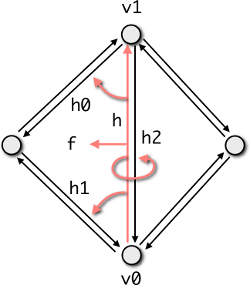
\includegraphics[width=0.3\textwidth]{content/media/sm_connectivity-queries}
  \caption{Surface\_mesh - Halfedge Verbindungen \cite{OpenGP.24.07.2015}}
  \label{fig:sm_halfedge}
\end{figure}

Da Surface\_mesh auch als Halfedge Datenstruktur implementiert ist, kann ähnlich effizient zu OpenMesh über die Kanten iteriert werden.
\autoref{lst:sm_iterate} zeigt einige Basisoperationen die möglich sind.
Die Operationen aus Listing~\ref{lst:sm_iterate} sind zum besseren Verständnis in \autoref{fig:sm_halfedge} gekennzeichnet. 

\begin{lstlisting}[style=myCppStyle, caption=Surface\_mesh - Basisoperationen, label=lst:sm_iterate]
Surface_mesh::Halfedge h;
Surface_mesh::Halfedge h0 = mesh.next_halfedge_handle(h);
Surface_mesh::Halfedge h1 = mesh.prev_halfedge_handle(h);
Surface_mesh::Halfedge h2 = mesh.opposite_halfedge_handle(h);
Surface_mesh::Face     f  = mesh.face_handle(h);
Surface_mesh::Vertex   v0 = mesh.from_vertex_handle(h);
Surface_mesh::Vertex   v1 = mesh.to_vertex_handle(h);
\end{lstlisting}

Um das Netz zu verändern oder zu editieren unterstützt die Datenstruktur high-level Operationen zum Verändern der Topologie.
Mit \emph{Edge Collapse}, \emph{Edge Split} und \emph{Edge Flip} kann das Netz geändert werden.
Die Operationen sind in \autoref{fig:sm_topology} dargestellt. 

\begin{figure}
    \centering
  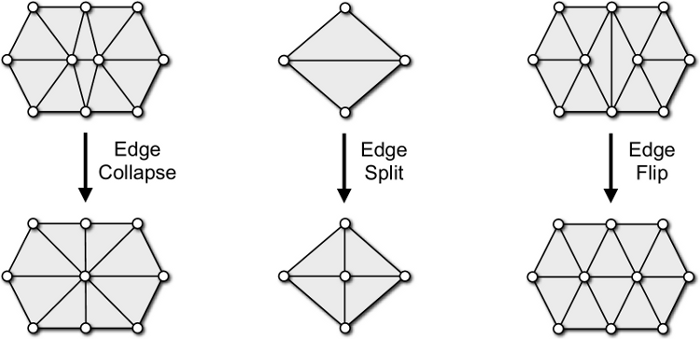
\includegraphics[width=0.8\textwidth]{content/media/sm_topology-changes}
  \caption{Surface\_mesh - high-level Operationen zum Ändern der Topologie \cite{OpenGP.24.07.2015}}
  \label{fig:sm_topology}
\end{figure}

Die Bibliothekt steht unter der \emph{GNU Library General Public License}, was eine problemlose Verwendung in diesem Projekt ermöglicht.

\subsection{OpenSubdiv}

OpenSubdiv wird von Pixar entwickelt und ist eine mächtige Bibliothek, die Unterteilungsalgorithmen und Datenstrukturen implementiert.
Die Bibliothek ist optimiert auf Performance und unterstützt paralleles Rechnen auf CPU und GPU.
Primär wird die Bibliothek von Pixar zum erstellen von animierten Filmen verwendet.
OpenSubdiv ist lizensiert unter der Apache License und darf somit frei für kommerzielle und nicht kommerzielle Projekt genutzt werden.

\begin{figure}
  \centering
  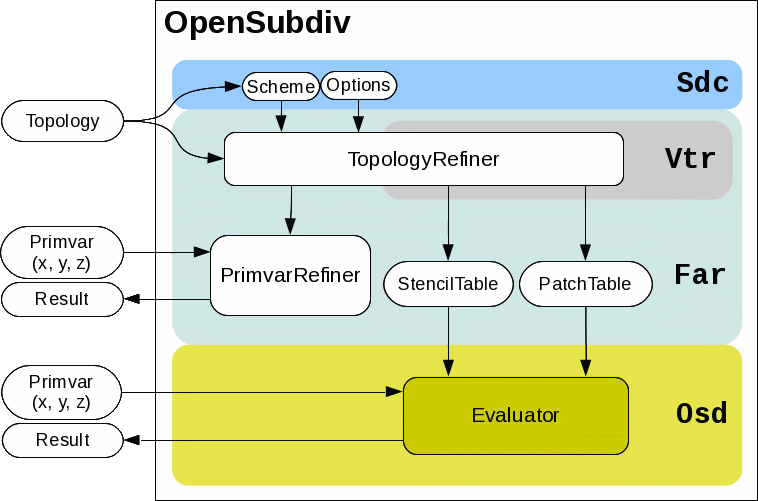
\includegraphics[width=0.9\textwidth]{content/media/pixar_opensubdiv}
  \caption{Pixar OpenSubdiv Architektur \cite{Pixar.27.07.2015}}
  \label{fig:pixar_opensubdiv}
\end{figure}

\autoref{fig:pixar_opensubdiv} zeigt den Aufbau der OpenSubdiv Bibliothek.
Sie besteht insgesamt aus den vier Schichten Sdc, Vtr, Far und Osd \cite{Pixar.27.07.2015}.

\begin{description}
 \item[Sdc] ist die unterste Schicht in der Architektur und implementiert die Unterteilungsdetails.
 Dazu gehören Typen, Optionen und Eigenschaften für die konkreten Unterteilungsalgorithmen.
 \item[Vtr] beinhaltet Klassen, die das Netz für effiziente Verfeinerung in einer Zwischenrepräsentation darstellen.
 Diese Schicht ist nur für den internen Gebrauch gedacht.
 \item[Far] ist die zentrale Schnittstelle, um Polygonnetze mit Unterteilungsalgorithmen zu verarbeiten.
 \item[Osd] beinhaltet geräteabhängigen Code, um Objekte aus der Schicht Far auch in unterschiedlichen Backends wie
  CUDA oder OpenCL ausführbar zu machen.
\end{description}

Von OpenSubdiv werden die Unterteilungsalgorithmen \emph{Catmull-Clark}, \emph{Loop} und \emph{Bilinear} unterstützt \cite{Pixar.27.07.2015}. 

\subsection{CGoGN}

CGoGN ist eine Geometric Modeling C++ Bibliothek und implementiert eine Datenstruktur für n-dimensionale Netze als Combinatorial Maps.
Diese Implementierung unterscheidet sich zu den Halfedge Datenstrukteren von OpenMesh und Surface\_mesh deutlich.
Diese sind zwar alle effizient, haben jedoch Probleme beim Umgang mit Objekten von unterschiedlichen Dimensionen.
Für jeden Problemfall muss die spezielle Datenstruktur verwendet werden.
All diese Strukturen lassen sich jedoch auf Combinatorial Maps zurückführen.
Diesen allgemeineren Ansatz geht CGoGN.
CGoGN implementiert bereits den Unterteilungsalgorithmus Catmull-Clark \cite{CGoGN.27.07.2015}. 

\subsection{Computational Geometry Algorithms Library (CGAL)}

CGAL ist ein mächtiges Softwareprojekt mit einer Vielzahl an Datenstrukturen und Algorithmen.
Neben Unterteilungsalgorithmen werden auch eine Reihe anderer Themengebiete abgedeckt (Voronoi Diagramme, Convex Hull Algorithms, Spatial Searching ...).
Für die Repräsentation von Netzen gibt es bei CGAL mehrere Möglichkeiten.

\begin{description}
 \item[Surface\_mesh] Zum einen implementiert CGAL die bereits vorgestellte Datenstruktur Surface\_mesh.
 \item[3D Polyhedral Surface] Neben Surface\_mesh kann auch die von CGAL entwickelte Halfedge Datenstruktur Polyhedral verwendet werden.
\end{description}

CGAL ist sehr mächtig und komplex. Die Bibliothek ist sogar in den meisten Paketquellen der Linux Distributionen enthalten (z. B. Ubuntu)
und kann darüber sehr leicht installiert werden.
Es sind auch bereits die Unterteilungsalgorithmen \emph{Catmull-Clark}, \emph{Doo-Sabin}, \emph{Loop} und \emph{Sqrt3} implementiert \cite{CGAL.27.07.2015}.

\subsection{Vergleich}

\autoref{tab:sd_bib} gibt einen Überblick über die vorgestellten Bibliotheken und listet auf, welche der ausgewählten Unterteilungsalgorithmen
(Catmull-Clark, Loop, Butterfly und Doo-Sabin) bereits implementiert sind.

\begin{table}
\center
\caption{Vergleich der Unterteilungsalgorithmus Bibliotheken}
\begin{tabular}{l|c|c}
\textbf{Bibliothek} & \textbf{Datenstruktur} & \textbf{Unterteilungsalgorithmen}\\
\hline
\textbf{OpenMesh} & Halfedge & Catmull-Clark, Loop, Butterfly\\
\textbf{Surface\_mesh} & Halfedge & keine\\
\textbf{OpenSubdiv} & Halfedge & Catmull-Clark, Loop\\
\textbf{CGoGN} & combinatorial maps & Catmull-Clark\\
\textbf{CGAL} & Halfedge & Catmull-Clark, Loop, Doo-Sabin\\
\end{tabular}
\label{tab:sd_bib}
\end{table}

Mit Ausnahme von Surface\_mesh, das wirklich nur die Polygonnetz-Datenstruktur mit elementaren Algorithmen implementiert, sind bei den anderen Bibliotheken bereits
einige Unterteilungsalgorithmen implementiert.
Bei Verwendung von OpenMesh oder CGAL könnte man sich viel Arbeit sparen, da dort schon fast alle gewünschten Algorithmen implementiert sind.
Ziel dieses Projektes ist jedoch eine einfache und schnelle Implementierung der Algorithmen.
Surface\_mesh selbst besteht nur aus wenigen Dateien und ist die schlankeste Bibliothek von allen vorgestellten.
\autoref{fig:surface_mesh_cmp} zeigt die Ergebnisse eines Benchmark-Vergleichs für die unterschiedlichen Datenstrukturen.
In dem Diagramm werden die Zeiten relativ zu Surface\_mesh angegeben.

\begin{figure}
  \centering
  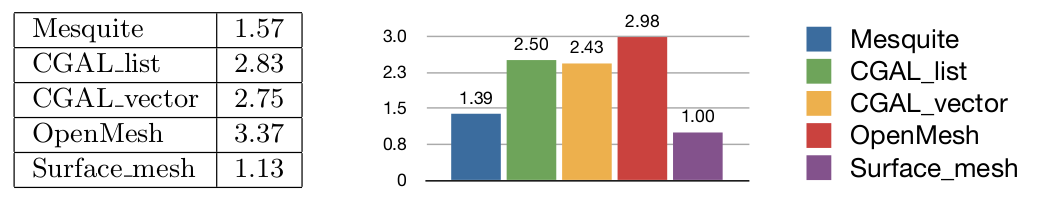
\includegraphics[width=1.0\textwidth]{content/media/surface_mesh_cmp}
   \caption{Benchmarks mit Surface\_mesh \cite{Sieger.}}
  \label{fig:surface_mesh_cmp}
\end{figure}

Man erkennt deutlich, dass die Datenstrukturen von CGAL und OpenMesh vergleichsweise langsam sind.
Da Surface\_mesh sehr kompakt ist (es besteht nur aus sehr wenigen C++ und H-Dateien) und in dem Benchmark auch sehr gute Ergebnisse liefert, fällt die Wahl auf Surface\_mesh.


\section{Rendering}

Im folgenden Unterkapitel werden Bibliotheken und bereits bestehende Software untersucht, mittels derer das Rendering von Polygonnetzen und Limesflächen realisiert werden kann.

Im Gegensatz zur großen Auswahl an unterschiedlichen Möglichkeiten wie beispielsweise bei den Datenstrukturen, beschränkt sich diese hier auf nur wenige Möglichkeiten. Die Wahl ist auf OpenGL wegen seinem großen Funktionsumfang und seiner weiten Verbreitung und auf BezierView auf Grund sehr guter funktionaler Überschneidungen gefallen.


\subsection{OpenGL}

Bei OpenGL handelt es sich um eine sehr weit verbreitete cross-platform Bibliothek für 2-D und 3-D Rendering.
Die API-Spezifikation von OpenGL beinhaltet eine Vielzahl von Befehlen, welche sowohl softwarebasiertes, als auch Hardware beschleunigtes Rendering auf der Grafikkarte ermöglichen. Das ermöglicht eine effiziente Umsetzung des Renderings von Polygonnetzen und Flächen.

Diese Effizienz zeigt sich beispielsweise auch bei Standardoperationen wie dem Draw-Call. Bedingt durch die Verwendung eines internen Zustandsautomaten muss der Befehl lediglich mit den veränderten Parametern aufgerufen werden. OpenGL-Befehle folgen einem konsistenten, sprachunabhängigen Namensschema, welches Informationen zum Aufruf und zur Funktionalität des Befehls enthält. So bezeichnet beispielsweise glVertex3fv() einen OpenGL-Befehl (gl), der einen Eckpunkt definiert (Vertex) und drei (3) float (f) Argumente als Zeiger (v) bekommt.

Ein weiterer Vorteil von OpenGL ist die Lizenzfreiheit für Anwendungsentwickler.

\subsection{BezierView}

NOCH GÜLTIG?

BezierView (kurz bview) ist ein einfaches Programm zum Rendern von Bézier Patches, rationalen Bézier Patches und Polygonnetzen 
\\\cite{Peters.bview.27.07.2015}.

Das Programm wurde von Saleh Dindar, Xiaobin Wu, Jorg Peters (University of Florida) entwickelt und ist für Forschungs- und Lehrzwecke als Open Source Projekt frei verfügbar. BezierView ist ebenso wie SubVis in C++ implementiert und verwendet OpenGL für das Rendering.

Überschneidungen ergeben sich besonders beim Rendern der Polygonnetze und der Limesflächen. Die Implementierung von BezierView kann als Grundlage für die konkrete Umsetzung von SubVis verwendet werden.


\section{Grafische Oberfläche}

In diesem Abschnitt werden die Bibliotheken, die für die Darstellung nötig sind, vorgestellt.

\subsection{Qt} 

\begin{figure}[hp]
  \centering
  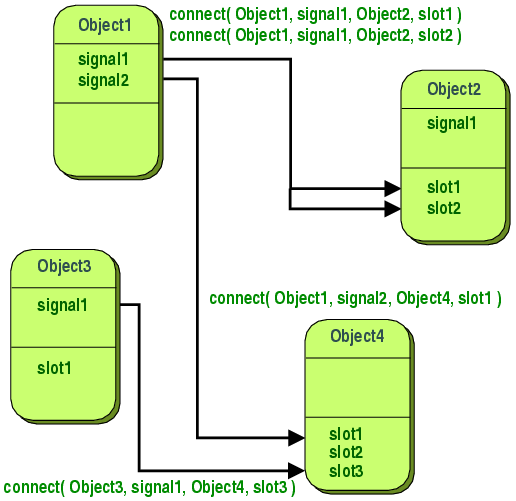
\includegraphics[width=0.6\textwidth]{content/media/qt_signal}
  \caption{Signal-Slots Konzept von Qt \cite{Qt}}
  \label{fig:qt_signal}
\end{figure}

Qt ist eine C++ basierte Bibliothek zur Entwicklung von grafischen Anwendungen \cite{Qt}. 
Der Vorteil von Qt besteht darin, dass die Anwendungen auf den verschiedenen Betriebssystemen annähernd nativ aussehen, in dem wann immer möglich, die nativen Widgets verwendet werden.
Eine Besonderheit von Qt ist das Signals-Slots Konzept (vgl. \autoref{fig:qt_signal}). 
Dieses kann als eine Art Beobachter-Entwurfsmuster betrachtet werden.
Dabei entspricht ein Signal einem \emph{notify} und ein Slot einem \emph{Beobachter}. 
Mittels einer \emph{connect} Funktion wird die Verbindung zwischen den Komponenten (n:m) hergestellt.
Zur Definition von Signalen und Slots werden Makros verwendet, die vom Meta-Object-Compiler \emph{moc} in standardkonformen C++ Code umgewandelt werden.

Es gibt die Möglichkeit das alte String-basierte Konzept oder das neue Zeiger-basierte Konzept (ab Qt 5) zu nutzen (siehe \autoref{lst:alt_signal_slots} und \autoref{lst:neu_signal_slots}).

\begin{lstlisting}[style=myCppStyle, caption={Altes Signal-Slots Konzept} \cite{QtWiki}, label=lst:alt_signal_slots]
connect(sender, SIGNAL (valueChanged(QString,QString)), 
	receiver, SLOT (updateValue(QString)));
\end{lstlisting}

\begin{lstlisting}[style=myCppStyle, caption={Neues Signal-Slots Konzept} \cite{QtWiki}, label=lst:neu_signal_slots]
connect(sender, &Sender::valueChanged, 
	receiver, &Receiver::updateValue);
\end{lstlisting}

Die neue Syntax ist eindeutiger, besitzt eine bessere Typprüfung zur Übersetzungszeit und erlaubt das Verbinden von Funktionen unabhängig davon, ob diese als Slot definiert wurden.

Qt wird unter der LGPL verteilt.

\subsection{libQGLViewer} 

Die Bibliothek bietet einige grundlegende Funktionen zur Erstellung von 3D OpenGL Betrachtern mit C++ \cite{libQGLViewer}.
Sie bietet unter anderem folgende Funktionen bzw. erleichtert deren Erstellung:

\begin{itemize}
\item Kamera ist im Raum frei positionierbar 
\item Weltkoordinatensystem
\item Verschiebung von Koordinatensystem und Objekten
\item Objektselektion mit der Maus
\item Screenshots
\item Tastaturkürzel und Maus-Bindings
\end{itemize}

Insbesondere das Konzept des \emph{Manipulated Frames} ist von besonderem Interesse für den Editiermodus. 
Es erlaubt, einen Frame dem Viewer zuzuordnen und auf diesem mit der Maus affine Abbildungen auszuführen.
Über die Methoden \emph{getPosition()} und \emph{setPosition(..)} kann die aktuelle Position im Raum abgefragt bzw. gesetzt werden.
Zu beachten ist allerdings, dass zu einem Zeitpunkt nur jeweils ein Frame pro Viewer gesetzt werden kann.
Somit muss bei mehreren beweglichen Objekten und damit Frames in der Anwendung manuell zwischen den Frames umgeschaltet werden.

Maus- und Tastaturtasten können beliebig neu belegt werden und somit vorhandene Funktionen eingeschränkt oder auf andere Tasten gelegt werden.
Dies ermöglicht eine optimale Konfigurierbarkeit auf den jeweiligen Verwendungszweck.

Um einen eigenen Viewer basierend auf der Bibliothek zu realisieren, muss lediglich die Klasse \emph{QGLViewer} erweitert werden.
Durch überschreiben der Methoden \emph{init()} und \emph{draw()} werden die anwendungsspezifischen OpenGL-Draw-Calls umgesetzt.

Gegenüber dem OpenGL Konzept einer festen Kamera \cite{OpenGLCamera} besitzt ein QGLViewer eine frei positionierbare Kamera, was intuitiver ist.
Das Kamera-Objekt kann ausgelesen und modifiziert werden, um die Kamera im Raum zu verschieben.

Die Software ist unter der GPL frei verfügbar.

\section{IDE} 

In Bezug auf Qt und C++ bietet sich die IDE \emph{Qt Creator} \cite{QtCreator} an. 
Diese bietet alle gewohnten Funktionen einer IDE wie Syntaxhervorhebung, Autovervollständigung, GUI-Designer, Debugger und Git-Integration.
Insbesondere der GUI-Designer nimmt viel Arbeit ab, da so einiges an Boilerplate-Code automatisch erzeugt werden kann.

Projekte werden in sog. \emph{.pro} Dateien konfiguriert. 
Diese Datei ist plattformunabhängig und relativ schlank gehalten. 
Erst bei Ausführung durch qmake wird ein plattformspezifisches Makefile generiert, welches dann mittels Make ausgeführt werden kann.

In der IDE können auch verschiedene sogenannte \emph{Beautifier} verwendet werden, welche den Quellcode formatieren.

\section{Quellcodeformatierung}

Ein weit verbreitetes Tool, um Quellcode zu formatieren ist \emph{Artistic Style (astyle)} \cite{astyle}.
Insbesondere in einem Projekt mit mehreren Entwicklern ist es sinnvoll, ein solches Tool zu benutzen, um einen einheitlichen Stil bezüglich der Formatierung zu erhalten.
Astyle bietet diverser vorgefertigte Stile an, erlaubt aber auch die feingranulare Definition von eigenen Stilen.
Die Konfiguration erfolgt entweder über Kommandozeilenparameter oder eine Options-Datei, welche eine bessere Übersicht bietet.
Astyle lässt sich im QtCreator über ein Plugin nutzen und einem Tastaturkürzel zuweisen.

\section{Dokumentation} 

Im Bereich C++ ist Doxygen \cite{Doxygen} eine weit verbreitete Quellcodedokumentationslösung.
Prinzipiell ähnelt es JavaDoc, in dem Quellcode direkt mittels spezielle annotierten Kommentaren versehen wird.
Diese Annotationen werden dann mittels Transformation in ein Ausgabeformat (z. B. HTML oder PDF) überführt.
Der Vorteil liegt darin, dass so die Dokumentation sehr nahe und eng mit dem Quellcode verbunden ist, was die Aktualität der Dokumentation begünstigt.
Qt Creator bietet Syntaxhervorhebung für die speziellen Kommentare und erleichtert so die Verwendung.

Doxygen steht unter der GPL.

\chapter{SubVis}

Nachfolgend wird das Programm \emph{SubVis} spezifiziert und dessen Architektur vorgestellt.
Außerdem werden die Entwicklungsorganisation, Dokumentation sowie verwendete Bibliotheken dargelegt.

\section{Anforderungen}

\begin{itemize}
 \item Architektur
 \begin{itemize}
 	\item Erweiterbarkeit durch andere Algorithmen mittels Plugins.
 	\item Plugins können eigene GUI-Elemente in dafür vorgesehenen Bereichen zeichnen.
 \end{itemize}
 \item GUI
  \begin{itemize}
 	\item Darstellung des Kontrollnetzes
 	\item Darstellung der Limesfläche
 	\item Rotation des Objektes
 	\item Translation des Objektes
 	\item Skalierung des Objektes
 	\item Beleuchtung der Oberfläche des Netzes, um Glattheit bewerten zu können.
 	\item Edit-Modus: Verschieben eines Punktes anhand seiner Flächennormalen.

 \end{itemize}
 \item Dateiformate / IO
 \begin{itemize}
 	\item OFF-Format und NOFF (mit Farben/Normalen)
 	\item Laden und Speichern von Polygonnetzen
 \end{itemize}
 \item Unterteilungsalgorithmen
 \begin{itemize}
 	\item Catmull-Clark
 	\item Loop
 	\item Doo-Sabin
 	\item Butterfly
 \end{itemize}
 \item Funktionen
 \begin{itemize}
  \item Variable Anzahl von Unterteilungsschritten
  \item Beleuchtungsmodus wählbar
 \end{itemize}
\end{itemize}

\section{Verwendete Tools und Bibliotheken}

\emph{SubVis} greift auf die Bibliotheken Qt, libQGLViewer, Surface\_mesh, OpenGL und Doxygen zurück.
Die verwendeten Versionen sind in \autoref{tab:versionen} ersichtlich.

Die genannten Versionen beziehen sich auf den jetzigen Zustand. 
Während der laufenden Entwicklung wird unter Umständen auf eine jeweils höhere Version aktualisiert.

\begin{table}[h]
\center
\caption{Versionen der Bibliotheken}
\label{tab:versionen}
\begin{tabular}{c|c}
Bibliothek & Version\\
\hline
Qt & 5.4.1\\
libQGLViewer & 2.6.1\\
Surface\_mesh & 1.0\\
OpenGL & 10.1.3-0ubuntu0.4\footnote{Ubuntu Paket mesa-common-dev}\\
Doxygen & 1.8.6\\
\end{tabular}
\end{table}

\section{Architektur}

Es wurde bisher die grundlegende Grob-Architektur festgelegt, welche definiert, welche Komponenten bestehen und wie diese miteinander kommunizieren.
In \autoref{fig:subvis_architektur} ist diese als UML-Komponentendiagramm dargestellt.

Grundsätzlich wird auf eine MVC Architektur gesetzt.
Die Model-Komponente soll die Datenstruktur mit dem Polygonnetz beinhalten und Import bzw. Persistenzoperationen anbieten.
Das Delegieren der Ereignisse aus der View-Komponente wird von der Controller-Komponente übernommen. 
Dort sollen auch die entsprechende Signale und Slots definiert werden.
Insbesondere die Editieroperationen werden an die MeshEdit-Komponente übergeben, welche dann die MeshData-Komponente ansteuert.
In der View-Komponente wird die GUI erstellt und gerendert. 
Deren Schnittstelle muss Operationen zum Erweitern der GUI und zum Beeinflussen des Renderings des Hauptfensters bereitstellen.
Auf diese Schnittstelle greifen dann die Plugins zu, die entsprechend eigene GUI-Elemente zeichnen und Plugin-spezifische Renderingmodi anbieten.

\begin{figure}
  \centering
  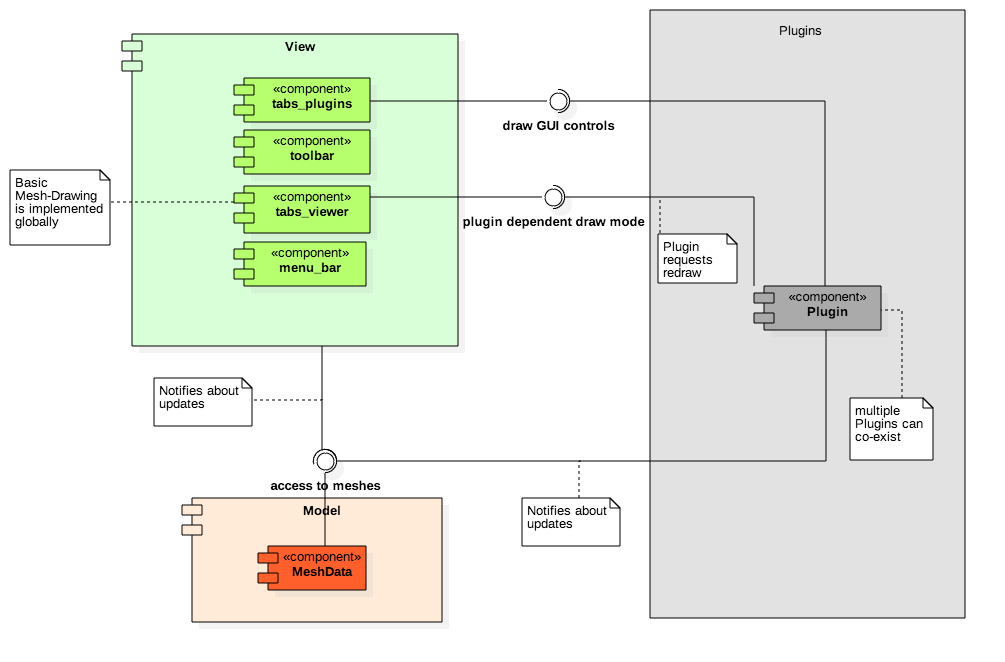
\includegraphics[width=\textwidth]{content/media/subvis_architektur.png}
  \caption{Geplante Architektur von SubVis}
  \label{fig:subvis_architektur}
\end{figure}

\section{Grafische Oberfläche}

Ein erster Entwurf der grafischen Oberfläche ist in \autoref{fig:subvis_gui_mockup} ersichtlich.
Während in der oben angeordneten Toolbar die allgemeinen Bedienelemente angeordnet sind, finden sich in der Plugin-spezifischen Seitenleiste die Einstellungen und weitere Optionen.
Die tatsächlichen GUI-Elemente in der Seitenleiste sind vom Plugin abhängig.

 \begin{figure}[hp]
  \centering
  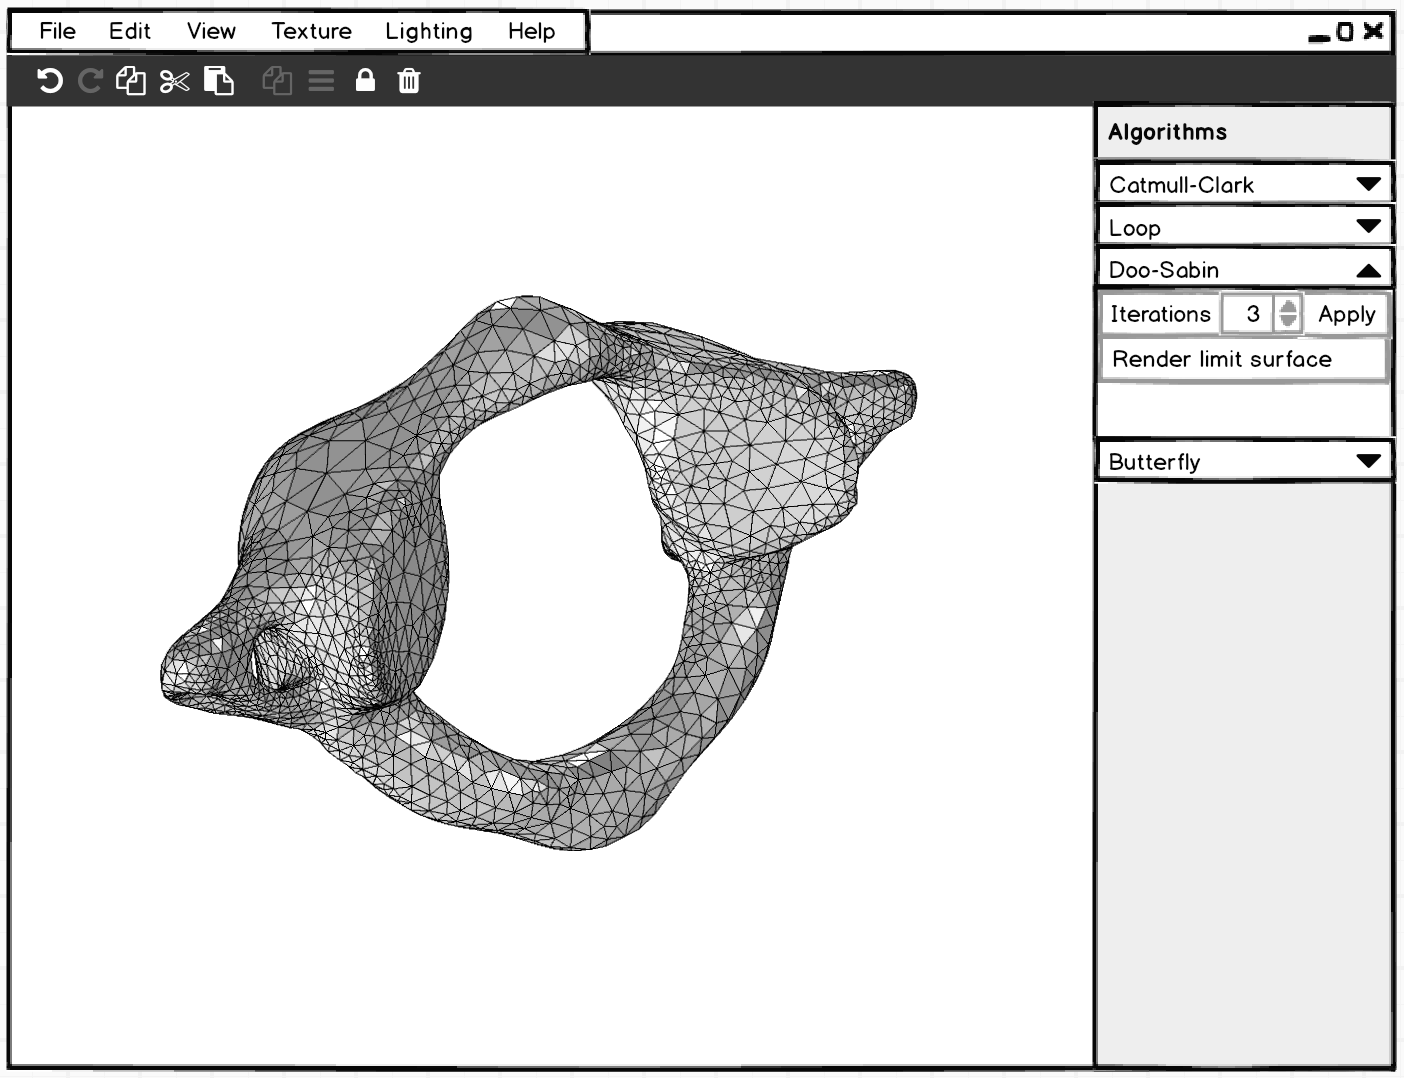
\includegraphics[width=\textwidth]{content/media/subvis_gui_mockup.png}
  \caption{Mögliche grafische Oberfläche von SubVis}
  \label{fig:subvis_gui_mockup}
\end{figure}

\section{Dokumentation}

Die Dokumentation besteht aus diesem Bericht sowie der finalen schriftlichen Ausarbeitung am Ende des 2. Semesters.
Diese Ausarbeitung soll die theoretischen Hintergründe erklären, sowie auf die Entwicklungsprozesse inkl. Vergleich und Entscheidungen für spezifische Technologien eingehen.
Ziel ist es, dem Leser eine Top-Down-Ansicht auf das Projekt zu verschaffen.
Es wird bewusst auf eine detaillierte Quellcodedokumentation in der Ausarbeitung verzichtet, um die Dokumentation nahe am Quellcode und aktuell zu halten.

Durch Quellcodedokumentierung sollen Entwickler befähigt werden schnell in das Projekt einsteigen zu können und das Programm weiter zu entwickeln bzw. durch Plugins zu erweitern.
Insbesondere bei den Plugins soll ein kurzes Tutorial erstellt werden, welches an die Plugin-Entwicklung heranführt. 
Des Weiteren soll ein kleines, gut dokumentiertes Plugin entstehen, um den prinzipiellen Aufbau zu veranschaulichen.
Wenn zu viel dokumentiert wird, veraltet diese schneller.
Deswegen soll \emph{sinnvoll} und \emph{angemessen} dokumentiert werden.
Dies bedeutet öffentliche APIs, wenn notwendig, detailliert und ausführlich zu dokumentieren und selbsterklärende Funktionen etc. nicht unnötig zu dokumentieren.
Grundsätzlich soll der Quellcode selbst schon als Dokumentation dienen können.
Zusätzlich finden sich beim Quellcode README-Dateien, die genaue Details über die verwendeten Funktionen, Build-Anleitungen und die Projektstruktur erläutern.

\section{Entwicklung}

Um eine gemeinsame Entwicklungsumgebung zu schaffen, wurden gewisse Bibliotheken, Tools und Plattformen spezifiziert.
Dies betrifft einerseits die Bibliotheken und Tools aus \autoref{tab:versionen}.
Andererseits auch das Betriebssystem, Versionsverwaltung, IDE und Programmiersprachenstandard.

Als Betriebssystem wird Ubuntu 14.04 LTS verwendet. 
Zum Projektabschluss wird jedoch eine plattformunabhängige Anwendung angestrebt.
Die Sprachfeatures von C++ sollen maximal dem C++11 Standard entsprechen.
Als Versionsverwaltung wird Git in Verbindung mit dem Git-Server des IOS an der HTWG eingesetzt. 

Die Entwicklung findet auf dem \emph{develop}-Branch und eventuellen  Feature-Branches statt.
Dabei sollte ein Branch pro Feature erstellt werden und erst dann in den develop-Branch gemergt werden, wenn das Feature funktioniert.
Als IDE wird der vorgestellte Qt Creator verwendet.

Das Projekt teilt sich in zwei Verzeichnisse auf: \emph{SubVis} und \emph{dev-doc}.
\emph{SubVis} enthält die gleichlautende Anwendung als Qt-Projekt und unterteilt sich noch in die Ordner \emph{app}, \emph{lib} und \emph{objs}.
\emph{app} enthält die Anwendungsteile die selbst entwickelt werden,
\emph{lib} die Drittherstellerbibliotheken und \emph{objs} 3D-Modelle zum Testen.
\emph{dev-doc} dient der weiterführenden Dokumentation.
Das Verzeichnis enthält z. B. Diagramme, diesen Bericht und andere hilfreiche Dokumente zur Entwicklung.

































\chapter{Projektverlauf}

In den folgenden Abschnitten wird der Projektverlauf beschrieben und ein Rückblick und Ausblick gegeben.
Es wird dabei auf die erreichten und geplanten Ergebnisse eingegangen, sowie der bisherige Ablauf des Projekts bewertet.

\section{Rückblick}

Im ersten Semester lag der Schwerpunkt darin, einen Überblick über die theoretischen Grundlagen zu erhalten. 
Hierzu gehören die Unterteilungsalgorithmen und die Darstellung der Kontrollnetze.
Ein weiter wichtiger Punkt war die Evaluierung von Bibliotheken, die bereits Algorithmen und vor allem Datenstrukturen implementieren. 
Als Ergebnis wurde die Datenstruktur Surface\_mesh als am geeignetsten bewertet.

Des Weiteren wurde die Architektur entworfen und in einem UML-Diagramm festgehalten.
Außerdem entstand eine einheitliche Entwicklungsumgebung basierend auf Qt und dem Qt Creator unter Ubuntu.
Diese enthält die nötigen Build-Dateien, Verzeichnisse, Bibliotheken und Git-Konfigurationen.
Jedes Teammitglied besitzt somit eine einheitliche, funktionierende Entwicklungsumgebung.
Zusätzlich wurde eine Dokumentationslösung auf Quelltextebene mittels Doxygen implementiert.

Da für alle Beteiligten der Umgang mit C++ und insbesondere Computergrafik ein neues Themengebiet darstellt, war ein ausführlicher theoretischer Einstieg in das Thema notwendig. 
Hierbei hat sich die Unterstützung durch Herrn Prof. Dr. Georg Umlauf und Pascal Laube als sehr hilfreich erweisen.
In den Projektbesprechungen wurden technische Details geklärt und der theoretische Hintergrund erläutert.
Erst durch Verstehen der Details bezüglich der Unterteilungsalgorithmen, des Renderings und der Anwendbarkeit der Unterteilungsalgorithmen auf verschiedene Kontrollnetze konnten die Tools und Bibliotheken entsprechend evaluiert werden.

Während des Semesters wurden lediglich für sehr kurze Zeiträume und eng eingegrenzte Themengebiete die Aufgaben zwischen den Teammitgliedern verteilt.
Dadurch wurde sichergestellt, dass eine gemeinsame Wissensbasis entsteht, um späteren Missverständnissen vorzubeugen.
Dies hat sich als hilfreich erwiesen und ermöglicht es nun an verschiedenen Teilmodulen der Anwendung parallel zu arbeiten.

\section{Ausblick}

Im kommenden Semester liegt der Fokus auf der Implementierung der einzelnen Komponenten des Programms.
Das Ergebnis umfasst das spezifizierte Programm \emph{SubVis} und eine schriftliche Ausarbeitung, die den Aufbau und die Umsetzung beschreibt und begründet.
Diese enthält zusätzlich eine Dokumentation die eine Top-Down-Ansicht liefert. 
Implementierungsdetails werden im Quellcode mittels Doxygen dokumentiert.

\subsection{Aufgabenverteilung}

\begin{table}
\center
\caption{Aufgabenverteilung unter den Teammitgliedern}
\begin{tabular}{c|c}
Arbeitspaket & Teammitglied\\
\hline
Architektur, Oberfläche, Entwicklungsumgebung & Simon Kessler \\
Rendering und Darstellung & Tobias Keh \\
Unterteilungsalgorithmen & Felix Born \\
\end{tabular}
\label{tab:aufgabenverteilung}
\end{table}

Für die Entwicklung werden die Themen und Aufgaben unter den Teammitgliedern in drei Arbeitspakete aufgeteilt.

\begin{description}
\item[Architektur, Oberfläche, Entwicklungsumgebung] Hierzu gehört die Oberfläche, Bedienung, Architektur inkl. Plugin-System und die Spezifikation einer Entwicklungsumgebung.
\item[Rendering und Darstellung] In diesem Arbeitspaket soll die Berechnung und Darstellung der Kontrollnetze und deren Limesfläche implementiert werden.
\item[Unterteilungsalgorithmen] Umfasst die Implementierung der vorgegebenen Unterteilungsalgorithmen.
\end{description}

\autoref{tab:aufgabenverteilung} zeigt die geplante Aufgabenverteilung für kommendes Semester.
Die Zuteilung der Arbeitspakete stellt lediglich einen Startzustand dar. 
Um jedem Teammitglied Einblicke in alle Aspekte zu ermöglichen und so auch den größten Lerneffekt zu erzielen, werden Teilaufgaben der Arbeitspakete ausgetauscht.
Der unterschiedliche Arbeitsaufwand wird kompensiert, in dem nach Fertigstellung eines Arbeitspaketes die entsprechende Person bei den anderen Arbeitspaketen weiter entwickelt.

\subsection{Zeitplan}

In den verbleibenden Semesterferien sollen die folgenden Arbeitsschritte durchgeführt werden.
Dabei wird nicht eine endgültige Implementierung angestrebt, sondern eine funktionsfähige prototypische Implementierung, die im kommenden Semester weiter optimiert und ergänzt wird.

\begin{itemize}
\item Architektur und Komponenten
\item GUI
\item IO-Funktionalität
\item Plugin-System
\item Affine Transformationen
\item Unterteilungsalgorithmen
\item Rendering des Kontrollnetzes
\item Beleuchtungsmodi des Rendering
\end{itemize}



% ============================ ENDE HAUPTTEIL

% ============================ LITERATURVERZEICHNIS

\begin{singlespace}
\printbibliography
\end{singlespace}

% ============================ ENDE LITERATURVERZEICHNIS



\end{document}